\begin{frame}[fragile]{Tutorial: One-site state basics}

\begin{columns}

\begin{column}[T]{0.45\textwidth}
\begin{onlyenv}<1->
\begin{lstlisting}[language=JuliaLocal, style=julia, basicstyle=\small]
Zp = ITensor([1, 0], i)
Zm = ITensor([0, 1], i)
Xp = ITensor([1, 1]/√2, i) 
Xm = ITensor([1, -1]/√2, i) 
\end{lstlisting}
\end{onlyenv}
\end{column}

\begin{column}[T]{0.6\textwidth}
\begin{onlyenv}<1-1>
$|Z+\rangle = \begin{bmatrix} 1 \\ 0 \end{bmatrix}$,
  $|Z-\rangle = \begin{bmatrix} 0 \\ 1 \end{bmatrix}$ \\
$|X+\rangle = \begin{bmatrix} 1 \\ 1 \end{bmatrix}/\sqrt{2}$,
  $|X-\rangle = \begin{bmatrix} 1 \\ -1 \end{bmatrix}/\sqrt{2}$
\end{onlyenv}

\begin{onlyenv}<2->
\vspace*{-0.4cm}
\begin{center}
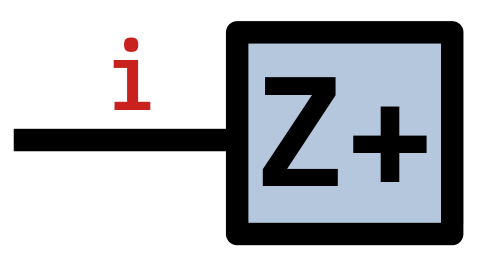
\includegraphics[width=0.3\textwidth]{
  slides/assets/Zp.png
}

\includegraphics[width=0.3\textwidth]{
  slides/assets/Zm.png
} \\

\includegraphics[width=0.3\textwidth]{
  slides/assets/Xp.png
}

\includegraphics[width=0.3\textwidth]{
  slides/assets/Xm.png
}
\end{center}
\end{onlyenv}
\end{column}

\end{columns}

\begin{columns}

\begin{column}[T]{0.45\textwidth}
\begin{onlyenv}<3->
\begin{lstlisting}[language=JuliaLocal, style=julia, basicstyle=\small]
(Zp + Zm)/√2
dag(Zp) * Xp
(dag(Zp) * Xp)[]
inner(Zp, Xp)
norm(Xp)
\end{lstlisting}
\end{onlyenv}
\end{column}

\begin{column}[T]{0.6\textwidth}
\begin{onlyenv}<3-3>
$\approx$ Xp \\
$\approx$ ITensor(1/√2) \\
$\approx$ 1/√2 \\
$\approx$ 1/√2 \\
$\approx$ 1
\end{onlyenv}

\begin{onlyenv}<4>
\vspace*{-0.4cm}
\begin{center}
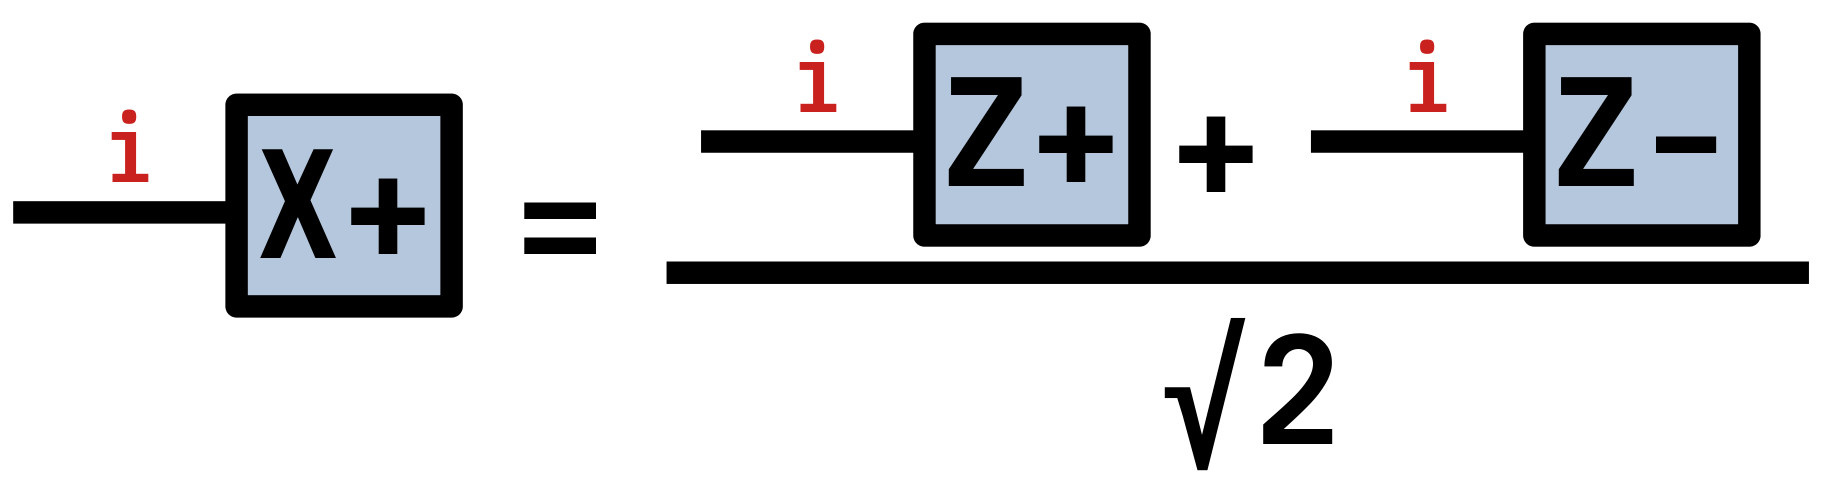
\includegraphics[width=1.0\textwidth]{
  slides/assets/Zp+Zm.png
} \\

\includegraphics[width=0.7\textwidth]{
  slides/assets/ZpXp.png
}
\end{center}
\end{onlyenv}
\end{column}

\end{columns}

\end{frame}
